\documentclass[a4paper,12pt]{article}
%\usepackage[magyar]{babel} 
\usepackage{t1enc}
\usepackage[utf8]{inputenc} 
\usepackage{lmodern}
\usepackage[pdftex]{graphicx}
\usepackage[lflt]{floatflt}
\usepackage{epstopdf}
\usepackage{amsmath,amssymb}
\usepackage{icomma} 
\usepackage{array} 
\usepackage[unicode,colorlinks]{hyperref} 
\usepackage{fullpage} 
\usepackage{booktabs} 
\usepackage{hhline}

\hypersetup{pdfstartview=FitH}

\title{\bf Monte Carlo methods \\ Exam replacement task \\ Documentation}
\author{ {Lázár György \tt (LIJIA8)}\\
}
\date{2022.\ 06.\ 10.} %A '\ ' paranccsal jelezzük, hogy ezek nem mondatvégi pontok, amik után alapból nagyobb köz kerül.

%Fattyú és árvasorok ellen
\widowpenalty=10000 \clubpenalty=10000

\newcommand{\tiz}{
\mathchar"013B
}

\newcommand{\me}[1]{
\,\mathrm{#1}
}

\newcommand{\cf}{
\me{^\circ C}
}

\newcommand{\gauss}[2]{
\left(\dfrac{\partial #1}{\partial #2}\right)^2\cdot (\Delta #2)^2
}
\newcommand{\deri}[2]{\frac{\mathrm{d}#1}{\mathrm{d}#2}
}
\newcommand{\E}[1]{\cdot 10^{#1}}
\begin{document}


\maketitle
\begin{abstract}
This document contains the brief description, usage, structure, of the particle transport simulation program. The software is written in the C language, and is based on a Monte Carlo method. This document also contains the results of a few experiments with the program, as well as the discussion for these.
\end{abstract}

\section{Basic information}
\subsection{Features}
\begin{itemize}
\item Multi-threaded structure, optimized for efficiency
\item Using \texttt{wyrand} - the quickest random number generator I could find
\item Easily expandable - the program is written in a way that new features (like new reactions) could be added easily
\item Safe memory management - Dynamic memory allocations do not happen in the computing core, reducing the possibility of a memory leak, and making the software more efficient
\item Usage of an external plotter - \texttt{gnuplot} - makes the compiled binary size very small and lightweight
\end{itemize}

\subsection{Dependencies}
\begin{itemize}
\item \texttt{POSIX} compatible environment - this includes all popular UNIX or UNIX-like systems. It is possible to use MinGW on non-\texttt{POSIX} compliant versions of Windows.
\item \texttt{[OPTIONAL]} gnuplot binary. Does not required for compilation, but it is a runtime requirement for real-time plotting (which can be disabled). Check \ref{nognuplot} for more information.
\end{itemize}

\subsection{Usage}
Basic usage requires a configuration file, which is passed as an argument to the software. If no configuration file is specified, the program will default to \texttt{config}. An example configuration file is provided, also named \texttt{config}. The structure of the configuration file is very strict, and the software does not give adequate debugging messages in most cases (missing feature), so please refer to the example configuration. Configuration options are the following.
\begin{itemize}
\item \textbf{Thread count:} Number of computing threads the software will use. Setting this higher than the thread count of the CPU will improve performance dramatically. At least 1 computing thread is required. The program will always run on at least 2 threads, since the main thread is separate.
\item \textbf{Channels:} Number of channels the data collector has.
\item \textbf{Stop when collisions reach:} The software will stop if this total number of counts is reached.
\item \textbf{Real time plotting with gnuplot:} 1 - real time plotting is enabled; 0 - real time plotting is disabled. If disabled, \texttt{gnuplot} isn't required to run the program. \label{nognuplot}
\item \textbf{Density (g/cm3):} Density of the detector material.
\item \textbf{FWHM:} FWHM of the detector.
\item \textbf{Energy of the source:} Energy of the mono-energetic source in keV.
\item \textbf{Update real time every N collisions:} Update the \texttt{gnuplot} chart every time a multiple of this number of total counts is reached. Has no effect if real time plotting is disabled.
\item \textbf{gnuplot executable:} Location of the \texttt{gnuplot} executable. If it's in \texttt{\$PATH}, leave this as is. Has no effect if real time plotting is disabled.
\item \textbf{Cross section file generated by xcom:} The output file with the cross sections, generated by the \texttt{xcom} program, as is.
\item \textbf{Save file:} The file which the output data in energy - counts format is saved, if the program finished execution. Leave this blank to disable saving the data.
\item \textbf{Particle source position:} Position of the particle source
\item \textbf{Cylinder (top,bottom,radius):} Parameters of the cylinder-shaped detector
\end{itemize}

\section{Program structure}
\subsection{Brief overview}
The software is written entirely in C. Uses the very fast random number generator, called \texttt{wyrand} from \texttt{wyhash} \cite{wyrandgit}. The program is split into a lot of modules. The \textit{random.h} is essentially a wrapper around \texttt{wyhash}, to easily access the \texttt{wyrand} algorithm, contained in \textit{wyhash.h}. The \textit{transport} module contains geometric calculations. The \textit{reactions} module computes reaction related numbers, such as cross sections, or reaction shuffling. It also contains a cache for the cross sections at the source energy, since this is needed a lot of times during the simulation. The module has to be initialized with \texttt{initReactions()}, and has to be freed via \texttt{freeReactions()}. The \textit{input} module handles the configuration file parsing. And finally, the \textit{tmath} module provides the vector struct, accompanied with the necessary operators. This last module was written by me, but at an earlier point in time, for another program, so that's the reason why it contains some unused functions.

The \textit{main.c} just welds these modules together. Thread handling, and plotting also happens in the main module. An important dilemma in multi-threaded applications, is how to evade race conditions - we don't want two threads to simultaneously write to the same memory address. The way I solved this problem is not the most efficient way. The C programming language does not support multi-threading natively, so the types required to create volatile variables are also not supported natively. So after the threads reach a given number of counts, they stop, and in the main module, their channels are summed up. After that, the threads are immediately restarted, and this data is plotted right after the main thread, so hopefully as little resources are used as necessary. If the threads are stopped on a "macroscopic timescale", this summation should have very little effect. The random collisions per thread should reach their maximum at about the same time. However, this is only true if every physical computing core in a given CPU is equal, which is not the case in modern smartphones, or even the M1/M2 Macbooks, or recent Intel CPUs - where so-called "big.LITTLE" core configuration is used instead. So in these cases, performance might take a quite noticeable hit, however, I am not familiar with how the operating system optimizes for these edge cases - starting a sufficiently large number of threads might make this unwanted phenomenon negligible.

The plotting happens via calling the \texttt{gnuplot} executable, and using \texttt{popen}, essentially piping the data into it. This would be very inefficient, however, the computing threads are running on other threads, while this process is handled by the main thread, so again, this should be negligible on the overall performance.

Another interesting thing I found out using \texttt{gprof} was, that the software was using incredible amount of computing resources for calculating the cross sections. I experimented a bit with it, like using an interval halving method for finding the required energy value in an array, but it didn't improve performance noticeably. What I found that had an effect however, is caching the cross section values for the source energy, which is most often required while tracing a particle's path.

\section{Tasks}
Here I will discuss the result of the given tasks.
\subsection{Task 1}
In task 1, we had to plot the spectrum in two separate configurations.
\subsubsection{A}
In task 1/A, the parameters, and the resulted spectrum were the following:
\begin{table}[h!]
\centering
\begin{tabular}{|l|l|}
\hline
Source position & (3,-3,2) cm \\ \hline
Source energy & 661.7 keV \\ \hline
Cylinder radius & 2.5 cm \\ \hline
Cylinder height & 3 cm \\ \hline
Detector density & 3.67 g/cm$^3$ \\ \hline
FWHM & 6 keV \\ \hline
\end{tabular}
\end{table}

\begin{figure}[h!]
\centering
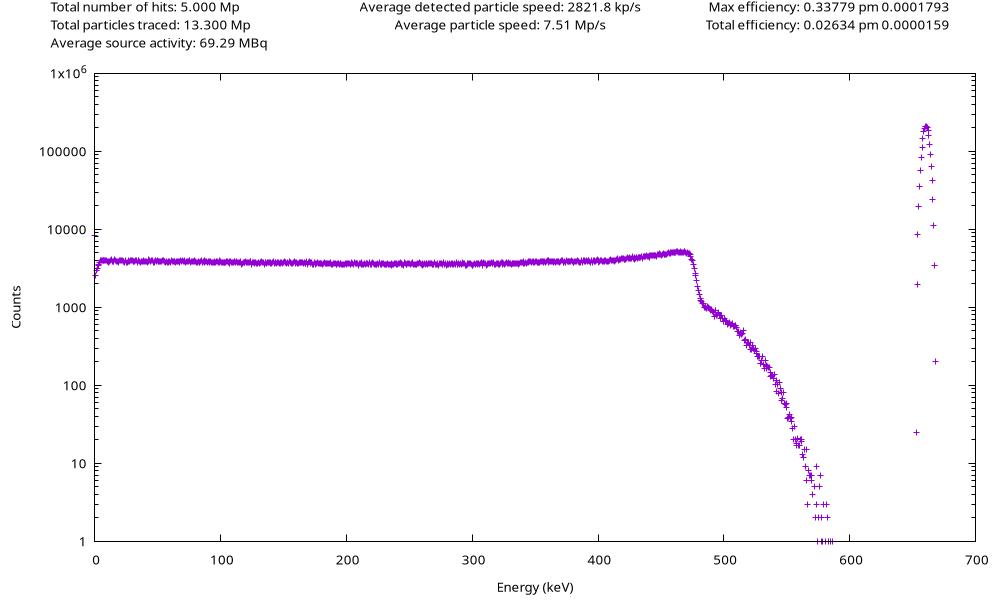
\includegraphics[width=\textwidth]{./1A.png}
\caption{Task 1A: Gamma spectrum via the given parameters.}
\end{figure}

\subsubsection{B}
In task 1/B the parameters, and the resulted spectrum were the following:
\begin{table}[h!]
\centering
\begin{tabular}{|l|l|}
\hline
Source position & (4,4,0) cm \\ \hline
Source energy & 1332.5 keV \\ \hline
Cylinder radius & 3 cm \\ \hline
Cylinder height & 5 cm \\ \hline
Detector density & 3.67 g/cm$^3$ \\ \hline
FWHM & 8 keV \\ \hline
\end{tabular}
\end{table}

\begin{figure}[h!]
\centering
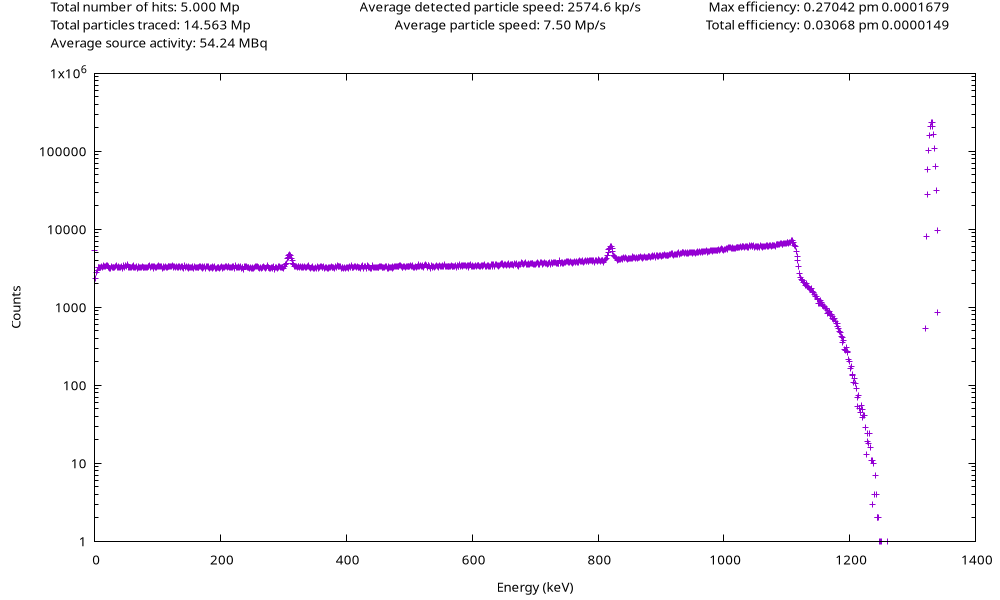
\includegraphics[width=\textwidth]{./1B.png}
\caption{Task 1B: Gamma spectrum via the given parameters.}
\end{figure}

In both spectra, certain characteristics are clearly visible, like the full energy peak, and the Compton edge, which are the basic building blocks of gamma spectroscopy. Particles with  energies between the Compton edge, and the full energy peak can also be observed - these are caused because by the high energy particles transfering only a small portion of their total energy via the multiple Compton effects.

In task 1/B, it is also noticeable, that there are some additional peaks on the Compton plateau. These are created thanks to pair production. The annihilating positron produces two photons with the energy of 511 keV. If one, or both photons escape, the initial particle from the source won't be able to dissipate all of the energy, so there will be additional peaks at the full energy peak, minus 511 and 1022 keV.

The Compton edges on spectrum A and B are at 474 and 1112 keV, respectively, which are very close to the theoretical values - 476.68 and 1118 keV. This is well within the margin or error of me determining, where does the Compton edge start exactly, so I can say with confidence, that the algorithm in my program to calculate the Compton effect is working well.

\subsection{Task 2}
In task 2, we had to work according to the parameters of 1/A, but the position had to be changed linearly between (1,3.5,2) and (-4,-1.5,2). The calculated efficiencies are plotted on \autoref{fig:eff1}, which is overlapping with our expectation. Both values increase with the distance between the source and the detector being reduced.
\begin{figure}[h!]
\centering
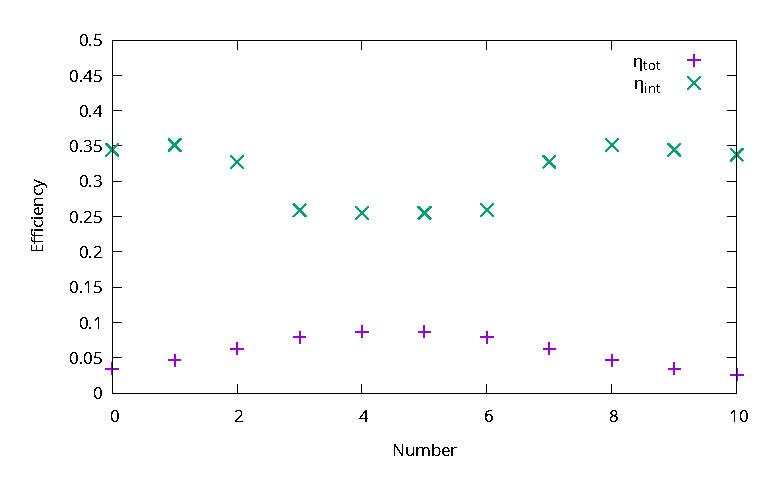
\includegraphics[width=\textwidth]{./2.eps}
\caption{Task 2: Efficiencies versus experiment number (varying the position)}
\label{fig:eff1}
\end{figure}

\newpage
\phantom{asdasd}
\newpage

\subsection{Task 3}
Task 3 was very similar to task 2, but instead of the position, we had to linearly increase the energy from 400 keV to 4MeV. The other parameters in this task had to be set according to 1/B. The results are plotted on \autoref{fig:eff2}, and it is also according to our expectations - increasing the energy does reduce the efficiency, but after a while, it is almost constant.

\begin{figure}[h!]
\centering
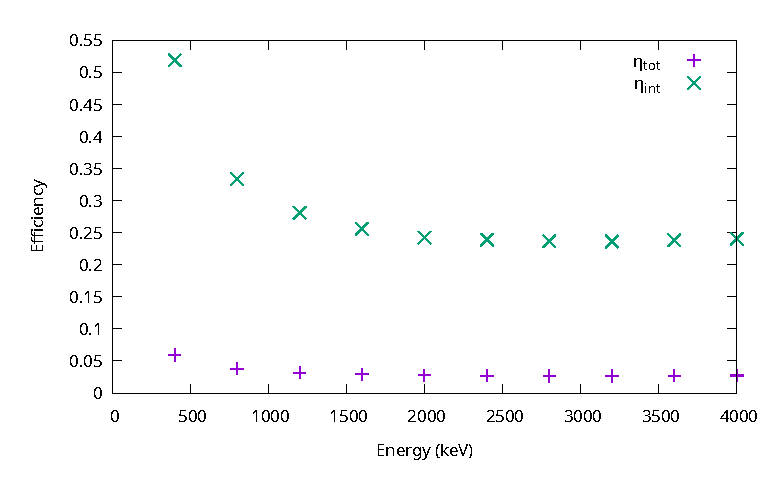
\includegraphics[width=\textwidth]{./3.eps}
\caption{Task 3: Efficiencies versus energy}
\label{fig:eff2}
\end{figure}

\section{Closing thoughts}
This project was pretty interesting, especially because I has to pick the programming language I'm working with. I chose C because it's a beautiful language, and gives you very fine-grained control over low-level things, like memory management. Matlab, in my opinion, is a cluttered, bloated dumpster fire, and I have no idea how did it become the industry standard in some places, so I tried to avoid it by any cost.

In the end, I also understand nuclear detector physics more. I got a lot more familiar with the subject, and now I can intuitively see a lot of things that I did not see before. So this project was not only great for my programming skills, but also was beneficial for my career in physics. In a way, this has a lot more sense, than an oral exam.

\begin{thebibliography}{1}
\bibitem{wyrandgit} Wyrand github page: \href{https://github.com/wangyi-fudan/wyhash}{https://github.com/wangyi-fudan/wyhash}
\end{thebibliography}

\end{document}